\section{Phase~2: Deep Learning Models}
\label{sec:phase2}

Phase~2 asks whether neural models improve on the Phase~1 Logistic Regression when they use the
same 59 leakage-safe features and the same day-ahead information. Four models were built: a simple
multilayer perceptron (MLP), a gated recurrent unit (GRU) network over daily delay
sequences~\cite{cho2014gru}, an MLP with learned categorical embeddings~\cite{guo2016entity}, and a
hybrid that feeds the embedding MLP's learned representation to XGBoost. Ablations measure what
each feature group and design choice contributes.

\subsection{Protocol}
Phase~2 follows the Phase~1 rules with one change of evaluation period. Each model is fitted on
January--July, its epochs and hyperparameters are chosen on August PR-AUC only, and it is refitted
on January--August for the chosen number of epochs. Encoders, scalers and vocabularies are refitted
on the training rows of each stage. Every model is then scored once on September--October (55{,}628
flights, delay rate 0.157), on exactly the same flights as the Phase~1 Logistic Regression. The
Logistic Regression was also selected on August, and calibration does not change its ranking, so
this is a fair comparison. November--December stayed sealed until one final model had been chosen.

Each neural model is trained with five seeds (42--46) and reported as mean $\pm$ standard deviation.
Differences in PR-AUC are tested with a paired bootstrap that resamples whole days (1{,}000
resamples), because flights on the same day share weather and congestion. A difference counts only
if its 95\% interval excludes zero. Each experiment plan was written into the decision log before
training.

\subsection{Models}
\textbf{Simple MLP.} The 49 standardised numeric features and 966 one-hot columns (1{,}015 inputs)
feed two ReLU layers of 128 and 64 units with dropout 0.3 and 0.2. All networks use Adam, an
unweighted binary cross-entropy loss and early stopping on August PR-AUC.

\textbf{GRU over daily sequences.} For a flight on day $D$, the model reads the previous $L$ days,
oldest first. Each day has ten values: the smoothed delay rate of the whole system and of the
flight's origin, carrier and destination; the log flight count of the system, origin and carrier;
a carrier has-data flag; and the weekday as sine and cosine. A past flight is counted on the day
its outcome became known (arrival plus 30 minutes, New York time), so a late arrival on day $D{-}1$
is not in day $D$'s sequence. A one-layer GRU reads the sequence, and its final state is joined
with the 59 static features before a 64-unit head. The grid $L \in \{7, 14, 28\}$ $\times$ hidden
size $\in \{16, 32\}$ selected $L = 14$ days and 16 units. A control model receives the same values
flattened, with no recurrence, to test whether reading the days in order matters.

\textbf{Embedding MLP.} Each of the 10 categorical features gets a learned embedding of dimension
$\min(c, \lceil\sqrt{v}\,\rceil)$ for vocabulary size $v$ and cap $c$, so the input shrinks from
1{,}015 to 86 values. A joint 48-run grid over learning rate, hidden layers, embedding cap, dropout
and batch size selected learning rate $10^{-4}$, layers (128, 64), cap 4, dropout 0.2 and batch
size 1{,}024.

\textbf{Ablations and hybrid.} The embedding MLP was retrained without the 29 historical features,
without the 4 scheduled-congestion features, with one-hot encoding instead of embeddings, and
without dropout and weight decay. The hybrid feeds the network's 64-unit last hidden layer, together
with the 49 numeric features, to XGBoost with the Phase~1 settings. A plain XGBoost was retrained
under the same protocol for comparison.

\subsection{Results on September--October}
Table~\ref{tab:phase2} and Fig.~\ref{fig:phase2boot} summarise the comparison. No Phase~2 model
ranks flights better than the Logistic Regression beyond bootstrap noise. The GRU has the highest
point estimate (+0.005), but its interval includes zero. The embedding MLP, the plain XGBoost and the
hybrid are reliably below it.

\begin{table}[htbp]
\centering
\caption{Phase~2 models on September--October (55{,}628 flights), mean $\pm$ sd over 5 seeds.
$\Delta$: PR-AUC difference from LR with 95\% day-bootstrap interval. ECE: October, after the
September sigmoid.}
\label{tab:phase2}
\resizebox{\columnwidth}{!}{%
\begin{tabular}{lcccc}
\toprule
Model & PR-AUC & ROC-AUC & ECE & $\Delta$ vs LR [95\% CI] \\
\midrule
LR (Phase~1) & 0.2896 & 0.680 & 0.027 & --- \\
GRU ($L{=}14$) & \textbf{0.2946} $\pm$ 0.0055 & 0.674 & \textbf{0.014} & $+0.005$ [$-0.014$, $+0.024$] \\
Simple MLP & 0.2839 $\pm$ 0.0043 & 0.672 & 0.024 & $-0.006$ [$-0.024$, $+0.012$] \\
Embedding MLP & 0.2757 $\pm$ 0.0035 & 0.675 & 0.030 & $-0.014$ [$-0.022$, $-0.003$]* \\
Plain XGBoost & 0.2681 $\pm$ 0.0055 & 0.672 & 0.030 & $-0.022$ [$-0.038$, $-0.004$]* \\
Hybrid DL + XGBoost & 0.2643 $\pm$ 0.0101 & 0.666 & 0.033 & $-0.025$ [$-0.039$, $-0.010$]* \\
\bottomrule
\multicolumn{5}{l}{* Interval excludes zero.}
\end{tabular}}
\end{table}

\begin{figure}[htbp]
\centering
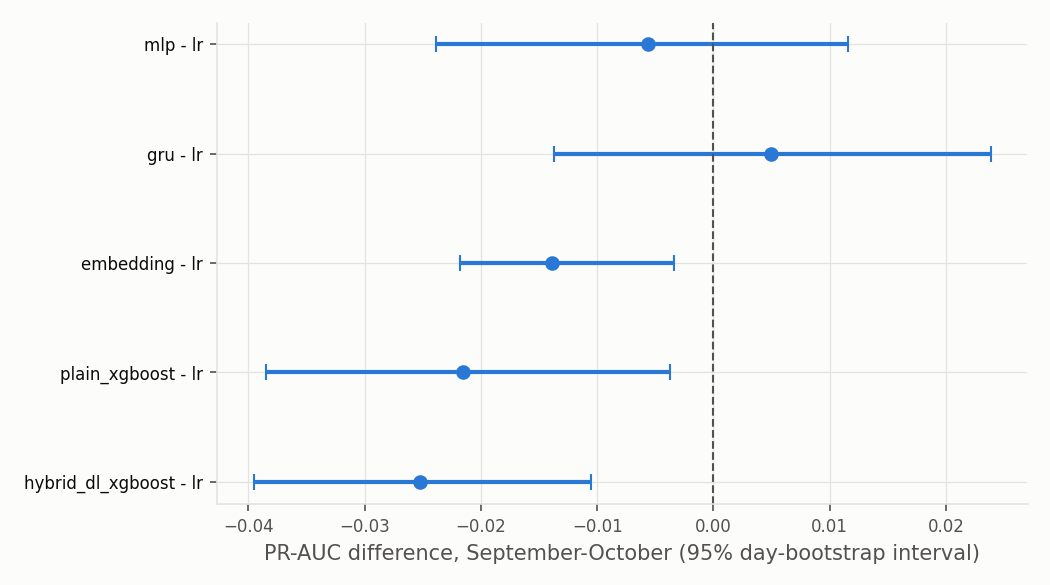
\includegraphics[width=\columnwidth]{phase2_bootstrap_vs_lr.png}
\caption{PR-AUC difference of each Phase~2 model from the Logistic Regression on
September--October, with 95\% day-bootstrap intervals.}
\label{fig:phase2boot}
\end{figure}

\textbf{Order matters.} The GRU beats its no-recurrence control by $+0.039$ [$+0.009$, $+0.072$],
so reading the days in sequence carries information that the same values in flat form do not. It is
ahead of the simple MLP by $+0.011$ [$-0.000$, $+0.022$], at the edge of significance. Removing the 29
historical features from the GRU changes PR-AUC by only $-0.006$ [$-0.022$, $+0.008$]: the sequence
recovers almost all of what the hand-built history features provide.

\textbf{Ablations.} Table~\ref{tab:ablation} compares each variant with the embedding MLP. Only the
scheduled-congestion features make a reliable difference. Removing the history features lowers the
mean by a similar amount, but its interval is wide because the effect varies from day to day.
One-hot encoding scores the same as embeddings, so the embeddings' advantage is a 12-fold smaller
input, not better ranking; they did not train faster (4--10 epochs against 2--3). Dropout and weight
decay make no difference, because early stopping after a few epochs already limits overfitting. The
hybrid is $-0.004$ [$-0.017$, $+0.008$] from plain XGBoost: trees on the learned representation do
not help.

\begin{table}[htbp]
\centering
\caption{Ablations of the embedding MLP (PR-AUC 0.2757), September--October}
\label{tab:ablation}
\begin{tabular}{lcc}
\toprule
Variant & PR-AUC & $\Delta$ [95\% CI] \\
\midrule
No congestion features & 0.2596 & $-0.016$ [$-0.027$, $-0.006$]* \\
No historical features & 0.2576 & $-0.018$ [$-0.046$, $+0.006$] \\
One-hot instead of embeddings & 0.2753 & $-0.000$ [$-0.006$, $+0.005$] \\
No dropout or weight decay & 0.2757 & $-0.000$ [$-0.003$, $+0.003$] \\
\bottomrule
\multicolumn{3}{l}{* Interval excludes zero.}
\end{tabular}
\end{table}

\subsection{Calibration, threshold and error analysis}
All models were calibrated with a sigmoid fitted on September and checked on October, as in
Phase~1. Calibration brings every model's October ECE to between 0.014 and 0.033, with the GRU
lowest (0.014, against 0.027 for the Logistic Regression). No threshold reaches 60\% precision for
the Logistic Regression or the embedding MLP. The GRU reaches it in all five seeds, flagging
160--358 October flights at a recall of at most 4\%. Other models that reach it do so by flagging as
few as one flight, so their thresholds are not usable.

For the error analysis, groups are compared by PR-AUC divided by their delay rate, because a random
ranking scores the delay rate and raw PR-AUC would simply favour busy groups. On October the hardest
carriers are FL (1.28 times random, but only 234 flights), AA and 9E; JFK is the hardest airport
(1.53, against 1.86 for EWR); and the hardest departure hours are 6~a.m.\ and 7~p.m. After the September calibration, every
model under-predicts flights leaving between 3~p.m.\ and 9~p.m., the busiest period of the day.

\subsection{Final model and single test}
The GRU was chosen as the single Phase~2 model for the test because it had the highest PR-AUC, the
best calibration and the only usable threshold on September--October. The choice, its saved
checkpoint (seed 42, the seed saved by design before any result), and its September calibration
and October threshold of 0.395 were committed and tagged before the test (D-312). The GRU was then
scored once on the same 53{,}991 sealed test flights as the Logistic Regression (D-313). Features
and daily sequences were built over the whole year using only past outcomes, and nothing was fitted
on the test period. Before scoring, the pipeline reproduced the GRU's saved September--October
probabilities bit-for-bit. Table~\ref{tab:phase2test} compares the two models.

\begin{table}[htbp]
\centering
\caption{Final comparison on the sealed test period, November--December (53{,}991 flights, delay
rate 0.258)}
\label{tab:phase2test}
\resizebox{\columnwidth}{!}{%
\begin{tabular}{llcccc}
\toprule
Model & Probabilities & PR-AUC & ROC-AUC & Brier & ECE \\
\midrule
GRU (Phase 2) & raw & 0.399 & 0.664 & 0.187 & 0.059 \\
GRU (Phase 2) & calibrated & 0.399 & 0.664 & 0.189 & 0.094 \\
LR (Phase 1) & raw & 0.398 & 0.664 & 0.226 & 0.204 \\
LR (Phase 1) & calibrated & 0.398 & 0.664 & 0.185 & 0.077 \\
\midrule
\multicolumn{6}{l}{At the frozen threshold, GRU: 1{,}102 flights flagged (2.0\%), precision 0.574,
recall 0.045.} \\
\multicolumn{6}{l}{LR: no threshold reached 60\% precision on October, so none was set.} \\
\bottomrule
\end{tabular}}
\end{table}

The GRU and the Logistic Regression rank test flights almost identically (PR-AUC 0.3986 vs 0.3979,
ROC-AUC 0.6638 vs 0.6640). No confidence interval was pre-registered for this comparison, so
neither model is claimed to be better. The frozen September calibration made the GRU worse
calibrated on the test period: ECE rose from 0.059 to 0.094, and the mean calibrated probability
was 0.164 against an observed delay rate of 0.258 (Fig.~\ref{fig:grureliability}). The cause is the
same calm-September effect seen for the Logistic Regression. The GRU's October threshold flags
2.0\% of test flights at 57.4\% precision, so the 60\% target, reached on October (in-sample), did
not carry over to the test period. The September--October advantages that motivated the choice did
not transfer.

\begin{figure}[htbp]
\centering
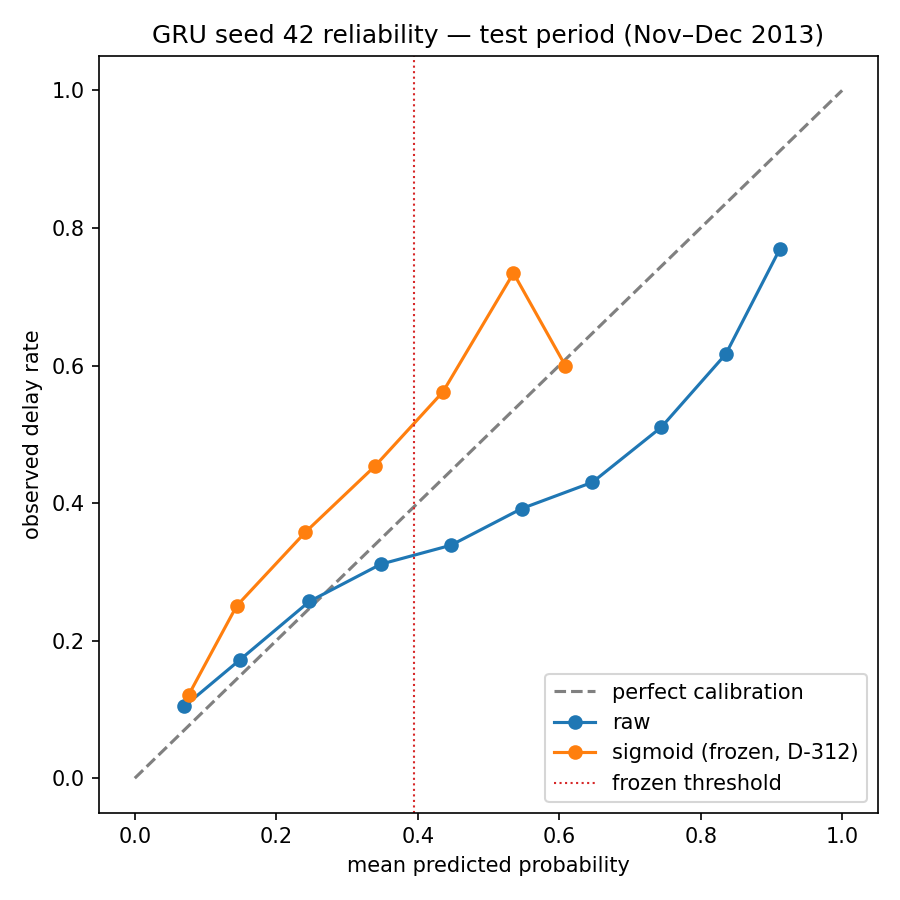
\includegraphics[width=\columnwidth]{phase2_gru_test_reliability.png}
\caption{Reliability diagram of the Phase~2 GRU on the test period, raw and with the frozen
September sigmoid. The dotted line marks the frozen October threshold.}
\label{fig:grureliability}
\end{figure}

\subsection{Discussion}
Five model families, from a linear model to a recurrent network and a tree--network hybrid, reach
almost the same ranking quality on the same inputs. This supports the Phase~1 reading: the limit is
the information available a day ahead, not model capacity. Phase~2 adds two structural findings.
The order of recent daily delays carries signal, and a GRU can learn most of the hand-built history
features from it. And scheduled congestion is the one feature group whose removal reliably hurts.
